\chapter{Elementos de la Web Semántica}
\label{chapter:semanticwebelements}

Aquí se presentará un panorama descriptivo acerca de la composición de la web semántica.

\section{Principios}

\subsection{Resource Description Framework (RDF)}

Es una familia de especificaciones de WC3 diseñada para modelar datos intercambiables en la web. 
Consta de expresiones hechas por tripletas. Cada tripleta es considerada una sentencia para este lenguaje.
Una tripleta es un conjunto de un valor de cada uno de los siguientes tipos:

\begin{description}
 \item[Recurso (sujeto)] Todo aquello descripto por RDF se lo denomina recurso, este último podría ser por ejemplo una página web entera (por ejemplo 
un documento HTML "http://www.w3.org/Overview.html") o una parte de ella.  Un recurso puede ser también un objeto que no 
se puede acceder directamente a través de la Web; por ejemplo un libro impreso. Los recursos son siempre nombrados por las 
URIs más identificadores de anclaje opcionales (ver [URI]). Cualquier cosa puede tener un URI; la extensibilidad de URIs 
permite la introducción de identificadores para cualquier entidad imaginable.
 \item[Propiedad (predicado)] Una propiedad es un aspecto específico, característica, atributo o relación se utiliza para describir un recurso. 
Cada propiedad tiene un significado específico, define sus valores permitidos, los tipos de recursos que se puede describir, 
y su relación con otras propiedades. 
 \item[Objeto] Puede ser otro recurso o puede ser un literal; es decir, un recurso (especificado por un URI) o una cadena simple o 
de otro tipo de datos primitivo definido por XML. En términos RDF, un literal puede tener contenido que es el formato XML,
pero no se evalúa aún más por el procesador de RDF.
\end{description}


Esta estructura forma una vinculación dirigida de un gráfico etiquetado, donde las aristas representan el enlace entre dos 
recursos (propiedad), representados por los nodos del grafo.

Su representación puede ser asociada tanto a un modelo entidad-relación como a un diagrama de clases de objetos.
Las Propiedades RDF pueden ser considerados como atributos de los recursos y en este sentido corresponden a pares 
atributo-valor tradicionales. Las Propiedades RDF también representan las relaciones entre los recursos y un modelo RDF,
por tanto, pueden parecerse a los de un diagrama entidad-relación.
En la terminología de diseño orientado a objetos, los recursos corresponden a los objetos y propiedades 
corresponden a las variables de instancia.

\subsection{RDF Schema (RDFS)}

Es una extensión semántica de RDF, que provee elementos básicos para la descripción de ontologías (también llamadas vocabularios RDF) con el objetivo
de estructurar los recursos RDF. Proporciona la manera de definir las clases y las propiedades específicas de la aplicación en RDF.
RDFS no proporciona las clases sino que proporciona el marco necesario para poder definirlas.

Clases en RDFS se parecen mucho a las clases en lenguajes orientados a objetos. Esto permite que los recursos se definan como 
instancias de clases y subclases de las clases.

\subsubsection{Elementos básicos}

\begin{itemize}
  \item 
    rdfs:Class permite declarar recursos como clases para otros recursos. 
    
    Atravez de la propiedad rdf:type, se puede asignar un tipo al recurso, un rucurso de tipo rdfs:Class puede entonces ser tipo de otro recurso. 
    Por ejemplo, podemos definir el recurso Auto como un rdfs:Class, y a su vez podemos definir el recurso Volkswagen Gol con la propiedad rdf:type 
    y siendo el objeto de esa propiedad el recurso Auto, entonces el tipo de Volkswagen Gol será auto.
    
    La defición de rdfs:Class es recursiva: rdfs:Class es la rdfs:Class de cualquier rdfs:Class.
  \item
    rdfs:Resource es la clase a la que pertenecen todos los recursos.
  \item
    rdfs:Literal es la clase de todos los valores literales, cadenas y enteros.
  \item
    rdfs:Datatype es la clase que abarca los tipos de datos definidos en el modelo RDF.
  \item
    rdfs:Property es la clase que abarca las propiedades.
\end{itemize}

\subsubsection{Elementos que definen relaciones}

\begin{itemize}
  \item rdfs:subClassOf es una instancia de rdf:Property (osea una propiedad) que permite definir jerarquías. Relaciona una clase con sus superclases.

  \item rdfs:subPropertyOf es una instancia de rdf:Property que permite definir jerarquías de propiedades.
\end{itemize}
    
\subsubsection{Restricciones de Propiedades}

\begin{itemize}
   \item rdfs:domain es una instancia de rdf:Property que especifica el dominio de una propiedad P. Esto es, la clase de los recursos que aparecen como sujetos en las tripletas donde P es predicado.

   \item rdfs:range es una instancia de rdf:Property que especifica el rango de una propiedad P. Esto es, la clase de los recursos que aparecen como objetos en las tripletas donde P es predicado.
    
\end{itemize}

\subsection{Vocabularios}

Son una colección de clases y propiedades con sus respectivas URIs, que son utilizadas para describir significado. Dichos vocabularios 
pueden ser fácilmente creados por cualquier usuario, sólo es necesario darle uso a la URI y documentarlo en algún lado. 
Por lo general, son estándares de uso no restrictivos de propiedades y clases que poseén una documentación.
El objetivo de los vocabularios es poder describir el significado de los recursos web y del mundo real, modelándolos en clases y 
propiedades que se utilizarán para describir al objeto en cuestión.

\subsection{OWL}


Web Ontology Languaje: Es un vocabulario que funciona como lenguaje para crear ontologías en la web. Fue creado en el 2006 y aceptado 
por WC3 como estándar en 2007 en su versión OWL 1.1. Tiene por objetivo proveer reglas a los vocabualrios para aumentar su expresividad. 
Estas reglas incluyen: jerarquías de clasess, cardinalidad, relaciones de conjunto, tipologías de propiedades más complejas, etc. Lo que proporciona la posibilidad de crear ontologías que pueden 
representarse en un paradigma muy parecido a la orientación a objetos. Cabe destacar que OWL no es el único vocabulario con este objetivo, ya que RDFS 
es también un conjunto de estándares mucho más básico que permite estas características.
En la actualidad existe la versión 2 de OWL que es mucho más completa.

\subsection{Ontologías}

La aparición de OWL permitió darle mucha más expresividad y restricciones a los vocabularios, que ahora no sólo eran un conjunto de 
propiedades y clases, sino que podían tener una definición mucho más completa, que permitía describir taxonomías y relaciones entre clases que pueden formar axiomas.
``An ontology is a formal specification of a shared conceptualization'' Tom Grubber (cita requerida)
Las ontologías se han convertido en uno de los pilares de la web semántica, esto se debe a que es uno de los principales componentes que permiten 
cumplir con el objetivo de ésta, que fue planteado en la introducción: ``La Web Semántica promete facilitar el desarrollo de la web social y la inteligencia colectiva, a través de mecanismos de clasificación, relación y descripción del contenido de la información publicada mejorando su interoperabilidad.''

\subsection{Motores de inferencias.}

Son componentes de software que pertimente establecer consecuencias lógicas en base a los axiomas definidos tanto por OWL como por RDFS
Estos componentes tienen como objetivo enriquecer las ontologías, creando reglas de inferencia. 
Dichas inferencias pueden ser más o menos complejas dependiendo de la capacidad y la configuración del motor utilizado. Existen tanto gratuitos 
como pagos.


\subsection{SPARQL}

Se trata de un lenguaje estandarizado de consulta de grafos RDF.
SPARQL se puede utilizar para expresar consultas que permiten interrogar diversas fuentes de datos (si es que los datos fueron almacenados 
de forma nativa como RDF o fueron definidos mediante vistas a RDF a travez de algún middleware). Tiene capacidades para la consulta
de los patrones obligatorios y opciones de grafo, junto con sus conjunciones y disyunciones. SPARQL también soporta 
la ampliación o restricción del ámbito de las consultas indicando los grafos sobre los que opera (grafos con nombre). Los resultados de las consultas
SPARQL pueden ser conjuntos de resultados o grafos RDF.

\subsubsection{Términos de conjuntos de colecciones de datos semánticos}

\begin{description}
 \item[Model:] Colección de sentencias.

 \item[DataSource:] Colección de Modelos. Siendo uno de ellos el modelo por defecto y el resto modelos con nombre. El Datasource es de lectura y escritura, por lo que se pueden agregar tripletas.

 \item[Dataset:] Lo mismo que el DataSource pero estático, por lo que es de solo lectura.

 \item[Graph:] Colección de tripletas. Cualquier modelo puede ser transformado a un grafo, y así tener una representación más cercana de RDF.

 \item[DatasetGraph:] Un contenedor de Grafos, similar al DataSource (También de lectura y escritura) que provee una estructura para un grafo por defecto y grafos con nombre.
\end{description}

\subsection{HTML semántico}

El uso y participación en la Web Semántica a travez de documentos RDF no es atractivo para la mayoría, porque no parece proveer un beneficio 
directo, ya que esto implica, aprender un lenguaje nuevo para generar documentos que sólo le será de utilidad a usuarios con un grado de conocimiento 
muy alto. 

Para resolver este problema, existen etiquetas de marcado en HTML que le proporcionan información semántica al documento, que copmo se verá más adelante 
puede ser extraída para generar documentos RDF. Existen distintos tipos:
\begin{description}
  \item[Microdatos:] Son un grupo de pares nombre-valor anidados dentro del documento, en paralelo con el contenido existente. Dichos grupo son 
también llamados ítems y cada par nombre-valor es la propiedad. Los atributos más utilizados son:
  \begin{itemize}
    \item itemscope: Se utiliza para crear un ítem
    \item itemprop: Se utiliza para crear una propiedad
    \item a, href, src, img: Se utilizan para definir valores URL
    \item value: Se utilizan para definir valores String
    \item itemtype: Se utiliza para establecer el tipo a un ítem.
  \end{itemize}

  \item[Microformatos:] Nacen con la intención acercar más personas al uso de la web semántica a travez de una forma sensilla de utilizar 
una serie de atributos de las etiquetas de XHTML:

  \begin{itemize}
    \item class: especifica el nombre de la clase

    \item rel: Se utiliza en los enlaces para indicar relaciones en los documentos.

    \item rev: Igual al rev pero en sentido inverso.
  \end{itemize}
  
Con el uso del atributo class se puede entonces especificar un microformato a utilizar. Existen muchos tipos como por ejemplo: hCard (para describir 
personas), hreview (para describir reviews), geo (para describir posiciones), etc. Cada uno de ellos con distintas propiedades.

\item[RDF-a:] Permite directamente embeber tripletas (sujeto-predicado-objeto) utilizando namespaces de XML. Modela la información en forma de grafo, 
a diferencia de microdatos y microformatos que lo hacen en forma de árbol, lo que hace que el mapeo a RDF sea claro, ya que en los otros casos puede ser problemático.
También tiene la opción de darle tipo a los literales. Como contrapartida tiene la desventaja de ser mucho más complejo de utilizar. 
\end{description}

\begin{figure}
    \centering
    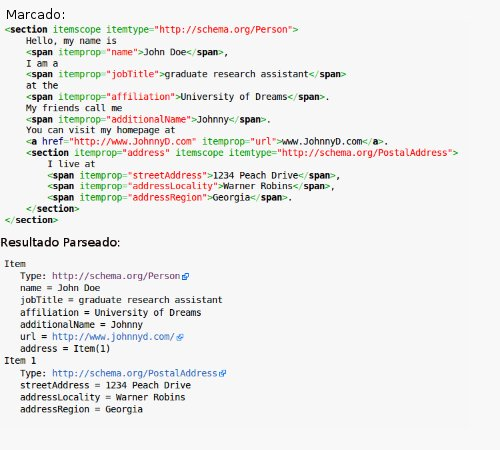
\includegraphics[width=0.8\textwidth,natwidth=610,natheight=642]{microdata}
    \caption{Ejemplo de marcado de microdatos y resultado}
\end{figure}
\begin{figure}
    \centering
    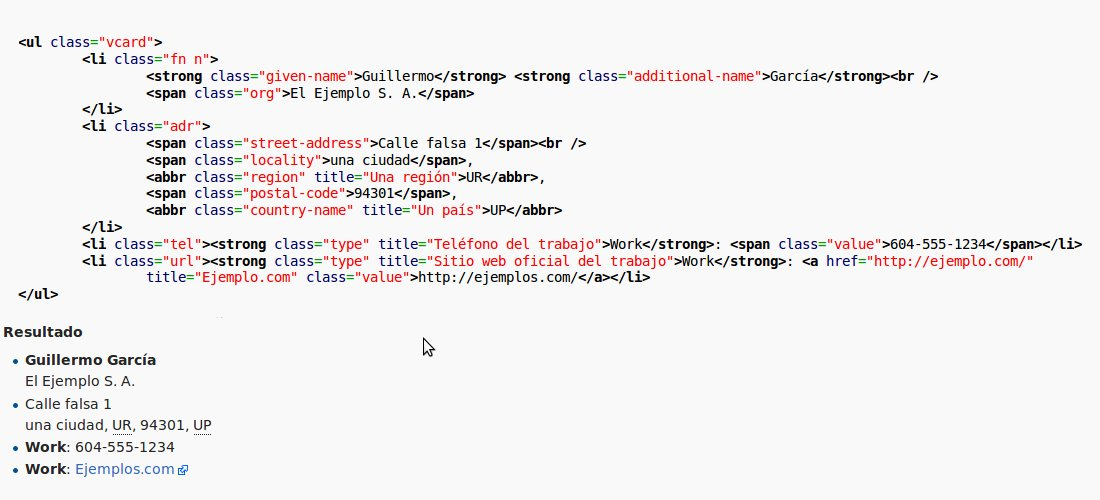
\includegraphics[width=0.8\textwidth,natwidth=610,natheight=642]{microformats}
    \caption{Ejemplo de marcado de microformatos y resultado}
\end{figure}
\begin{figure}
    \centering
    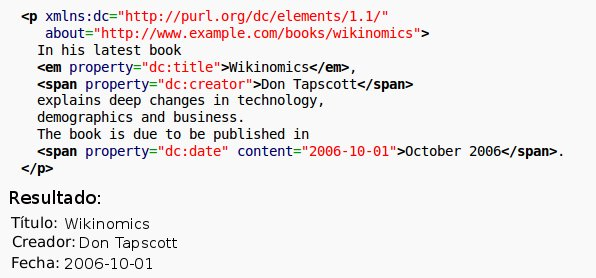
\includegraphics[width=0.8\textwidth,natwidth=610,natheight=642]{rdfa}
    \caption{Ejemplo de marcado de rdf-a y resultado}
\end{figure}

\subsection{Extractores}

Son herramientas que permiten extraer tripletas de los lenguajes de metadatos semánticos embebidos en HTML vistos anteriormente. 
Utilizan estándares como GRDDL, parseando todo el documento HTML y buscan sentencias para traducir a RDF y generar un nuevo documento 
que contiene sólo las tripletas de información semántica. 
Muchas veces (sobre todo con microformatos) los extractores tienen que tomar decisiones sobre cómo traducir a RDF, por lo que 
un mismo documento HTML puede ser extraído de distintas maneras según el extractor. Esto no ocurre con RDFa, ya que la equivalencia a RDF es mucho 
más clara.

\subsection{Dublin core}

Es un vocabulario ampliamente utilizado para describir tanto recursos web como recursos físicos creado en 2012. Comenzó siento un conjunto de 15 
propiedades 

\begin{lstlisting}
    Title		Publisher	Format
    Creator		Contributor	Identifier
    Subject		Date		Source
    Description		Type		Language
    Relation		Coverage	Rights
\end{lstlisting}



Consta también de Dublin Core Metadata Initiative que provee un foro de desarrollo de estándares de metadatos interoperable.
En la actualidad, se ha extendido a 55 propiedades y 22 clases.



\section{Aplicaciones en la Web Semantica}

\subsection{DBpedia}

La aplicación más importante de la Web Semántica, que tiene como objetivo extraer información de wikipedia, y crear una versión semántica 
de la información. Para ello creó una serie de ontologías, donde modelan y relacionan la información extraída de wikipedia.

Dbpedia en la actualidad es reconocido como el sitio autoritativo de recursos de la web semántica, siendo las URIs de estos recursos 
la mejor forma de identificarlos.
Es por eso que la gran mayoría de las aplicaciones de la web semántica utilizan la información de dbpedia para enriquecer sus datasets.
En Septiembre de 2013, se contaron mas de 45 millones de links entre DBpedia y datasets externos como  Freebase, OpenCyc, UMBEL, GeoNames,
Musicbrainz, etc.

\begin{figure}
    \centering
    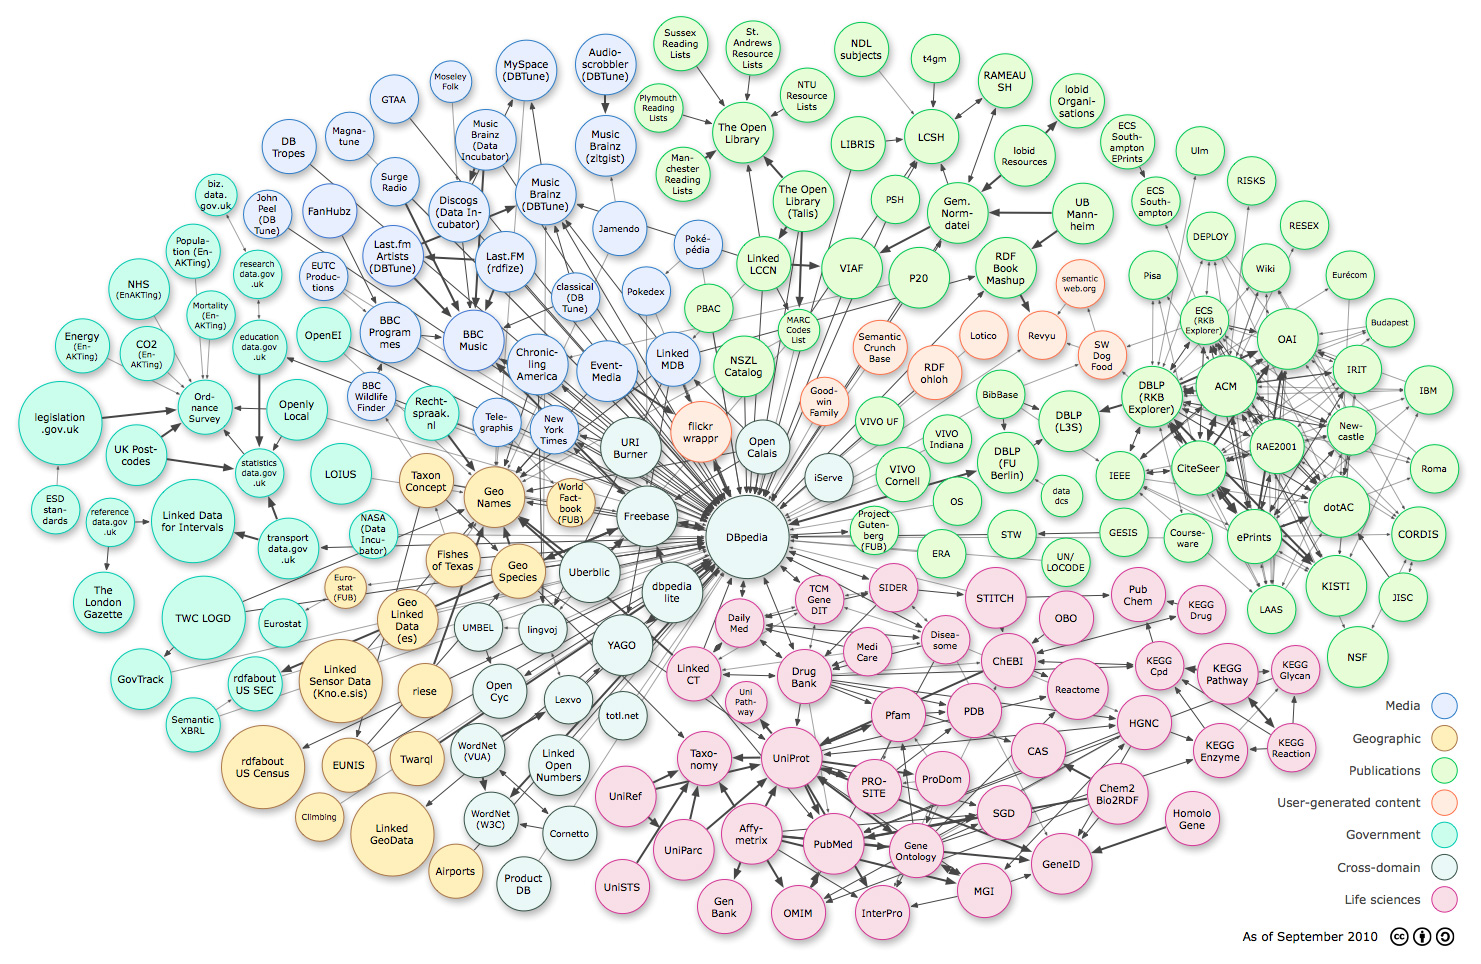
\includegraphics[width=0.8\textwidth,natwidth=610,natheight=642]{dbpedia}
    \caption{La utilización de DBpedia como fuente de datos}
\end{figure}

\subsection{Revyu}

Es una aplicación que se utiliza para publicar reviews de cualquier tipo en RDF. Alentando al usuario a generar reviews en la Web Semántica 
sin la necesidad de conocimiento sobre la misma.

Tiene el objetivo de proveer información reusable para otras aplicaciones, y generar datos de confianza y recomendación en las redes sociales.

La información es publicada tanto en documentos HTML como RDF además de su SPARQL Endpoint, siendo así de utilidad para los distintos tipos de usuarios.
También alienta el uso de links a distintos dataset semánticos, como el de DBpedia, RDF Book Mashup, etc.

\subsection{Sindice} 

Es una herramienta creada en conjunto por la Universidad de Deri,  Fondazione Bruno Kessler y Openlink Software que propociona 
múltiples tipos de API ofreciendo acceso a su dataset de la web de datos. 

Este dataset contiene información recolectada de la web en múltiples formatos de la web semántica y puede ser accedido a travez 
de un search engine, una API restful o un SPARQL endpoint. 

En la actualidad posee indexados 708.26 millones de documentos.

\subsection{Link Open Data Cloud Cache (LOD)} 

Al igual que sindice proporciona acceso a un dataset recolectado de la web de datos pero de una manera mucho más restringida. 

Se dispone de un text search (funciona como un search engine) o de un SPARQL Endpoint muy poco flexible y limitado en cuanto a 
la cantidad de información ofrecida comparada con la que podría ofrecer. Sólo se puede acceder al dataset entero mediante federated
queries, en caso de querer buscar sobre todo el dataset, el endpoint limita la consulta sólo a una parte del mismo. 

Tambien posee muchas restricciones respecto a los time outs, por lo que las consultas no pueden ser muy flexibles.
Para poder disponer de la funcionalidad completa del endpoint y así poder aprovechar tanto el dataset como las consultas SPARQL 
deberá comprarse una licencia.


\section{Tecnologías}

\subsection{Apache Jena}

Es un framework de Open Source para Java que permite crear aplicaciones de Web Semántica y Linked Data. \\
Proveé todas las funcionalidades necesarias para extraer, crear y publicar documentos RDF. Tiene soporte además para múltiples otros 
formatos de la web semántica. \\
También proporciona la posibilidad de crear dataset semánticos y utilizarlos mediante código en Java o a travez de un procesador SPARQL 
llamado ARQ.\\
Incluye además, opciones de serialización de grafos RDF a bases de datos relacionales.

\subsection{JSON Simple}

Es una pequeña librería para Java que permite una fácil y rápida serialización de objetos a 
Strings de JSON.

\subsection{Jersey}

Framework para Java que proveé una API que extiende las herramientas JAX-RS que simplifican el 
desarrollo de una API Restful. 
